\documentclass{article}
\usepackage{graphicx}     

\usepackage[hidelinks]{hyperref}
\usepackage{float}

\title{MIT 16.4400 Computer Graphics Project Proposal}
\author{David Berthiaume}

\date{\today}

\begin{document}
\maketitle
\tableofcontents

\section{Background}
One of my most vivid memories from my very early childhood is staring intently into a painting on the wall at the town library. This painting depicted
an aerial view of the town where I grew up. While the layout of the town was true to life, the colors
and details were starkly different. The painting represented a fascinating mix of real-world data and artistic interpretation. This project will attempt to create such an artwork from a unique geometric perspective using ray tracing.

\begin{figure}[H]
      \caption{Conceptual drawing of proposed rendering}
      \label{fig:con}
      \begin{center}
            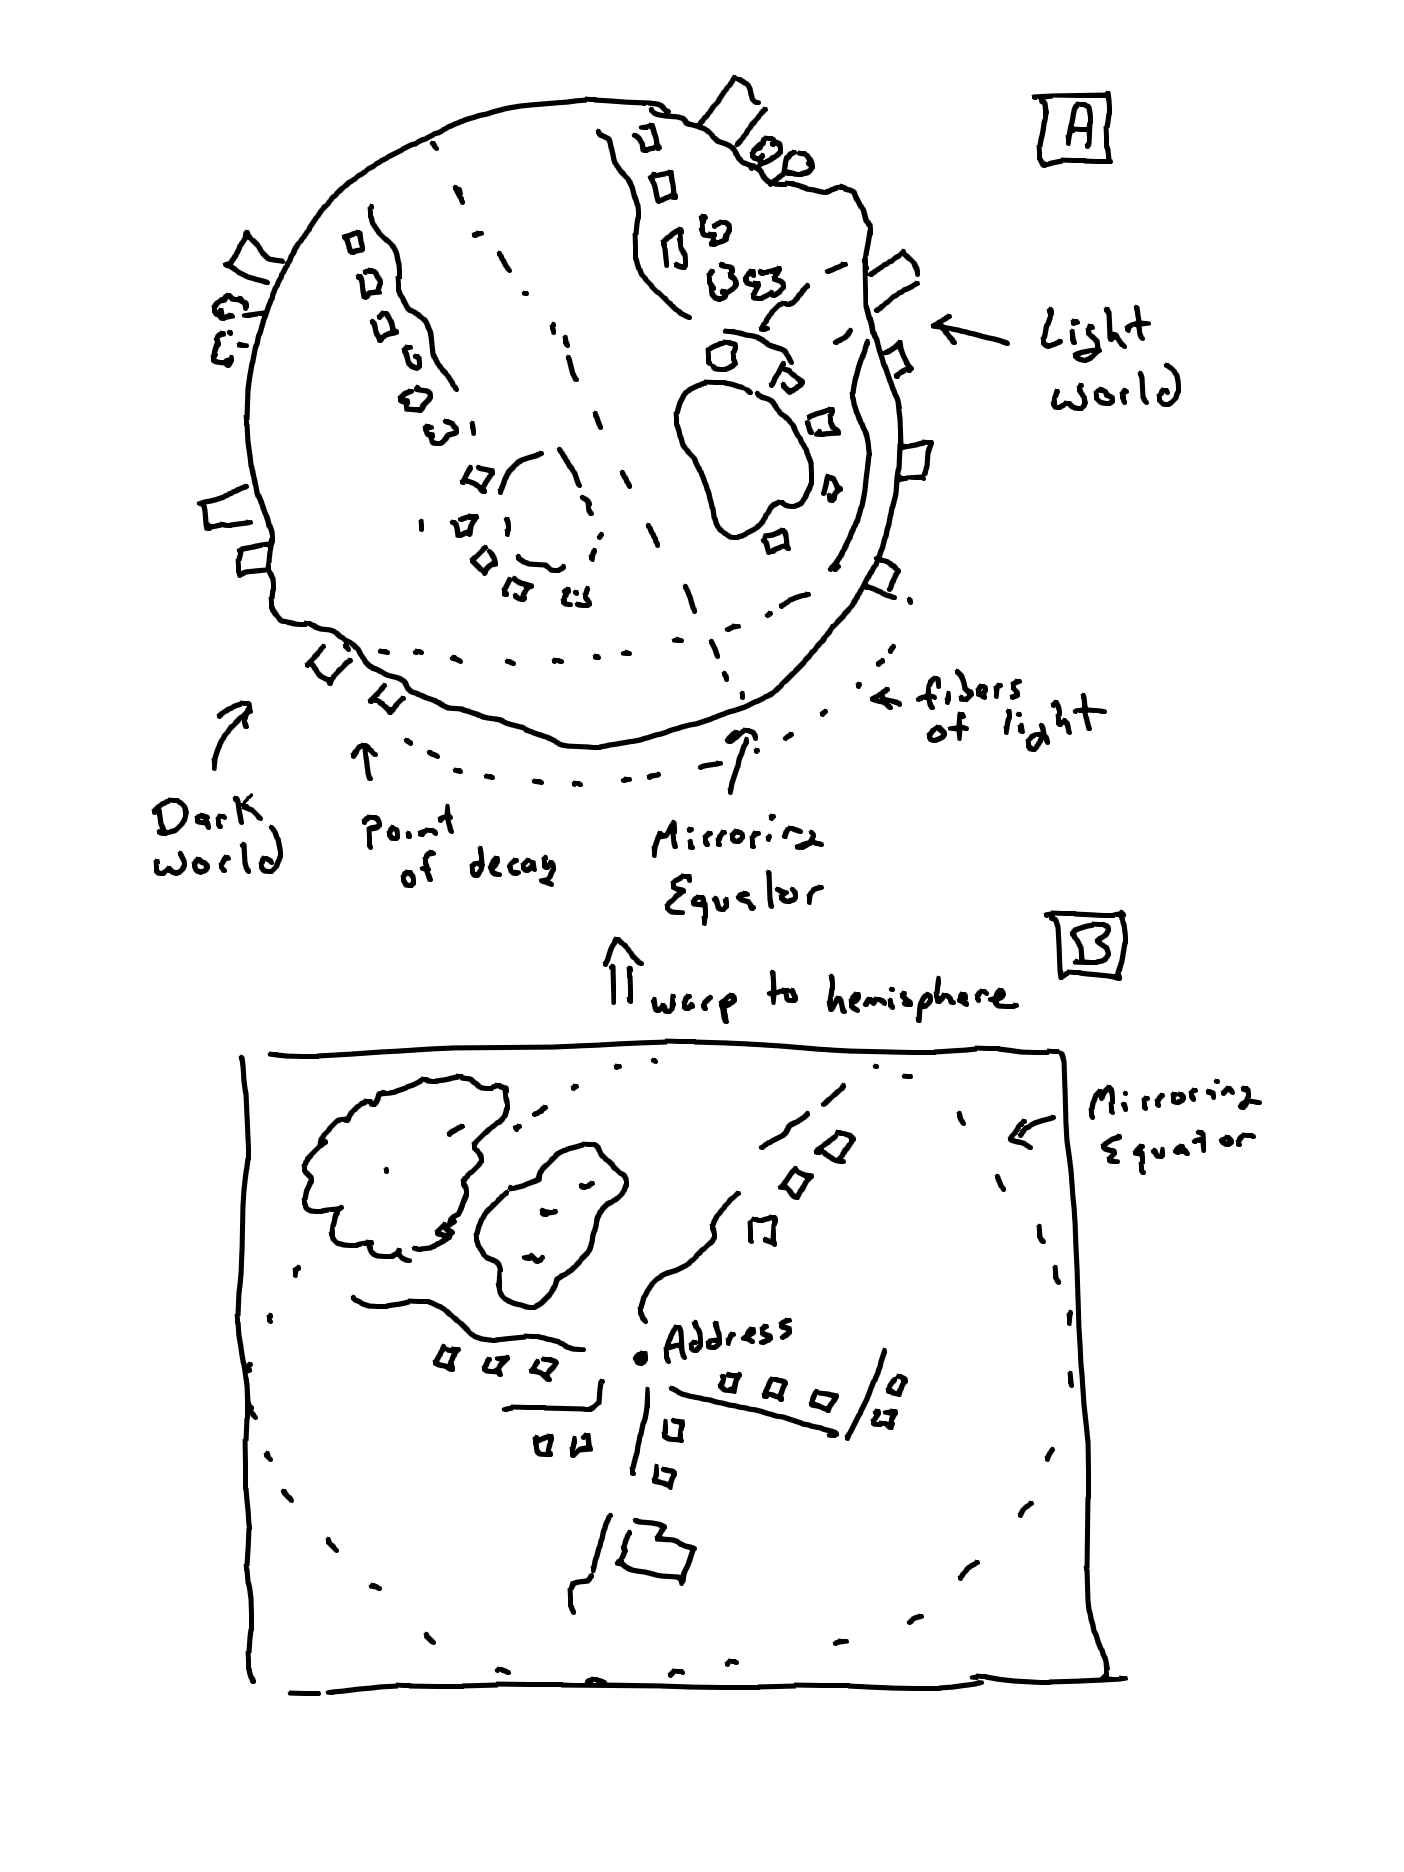
\includegraphics[width=4.5in]{conceptual_drawing.png}
      \end{center}
\end{figure}


\section{Project Description}
For this project, I will render a small planet using a custom ray tracer from scratch built in python. See figure \ref{fig:con}.
The terrain, roads, buildings, trees, and other objects, time permitting, will all
be based on real-world data, derived from various Massachusetts geospatial data sources. A disc of radius roughly 1km
of this data, projected onto a hemisphere will be used to create the geometry for each half of the planet.

There will be a light side of the planet and a mirrored dark side of the planet. The dark side will contain a reflection of the geometries on the light side with some artistic changes. Fibers of light that look like power lines providing illumination will connect the buildings from one side of the planet to the other.

A user will enter an address for any property in Massachusetts. A planet will be rendered with a central focus on that location. The final result will be a high-quality rendered image with antialiasing.

\section{Project Outline}

This project will consist of the following steps. Given the scope of this project, I started early, and steps 1, 2 and 3 have already been completed. Significant progress has been made on step number 4 and 5.

\begin{enumerate}

      \item Gather, process, clean, index, and organize around 800 GB of geospatial data for the entire state of Massachusetts, including LiDAR-derived bare-earth elevation data, land cover and use data, building footprints, imperviousness, and tree cover.
      \item Geocode the input address and produce a hemisphere of real-world data from the above repository by clipping and projecting each data set.
      \item Create a unified, coregistered raster at a resolution of 25cm/pixel from the above clipped data sets.
      \item Place trees and other objects based on sampling of the land use types through gridded placement, perlin noise, and then jittering. Extrude 2D buildings to create 3D shapes. Project these onto the hemisphere.
      \item Tessellate the heightmap into two hemispheres at 25cm resolution and assign materials.
      \item Create a ray-tracer from scratch in Python and numpy to render this planet using displacement mapping or tessellation. Use simple geometries to render the trees and other objects.
      \item Reflect the geometry across the equator to generate the dark side of the planet. Apply material and geometric changes to this dark hemisphere.
      \item Create the fibers of light connecting the buildings and implement indirect illumination.

\end{enumerate}


\section{Screenshots of Current Progress}

\begin{figure}[H]
      \caption{Cleaning, processing, registering, and clipping of land-use data}
      \begin{center}
            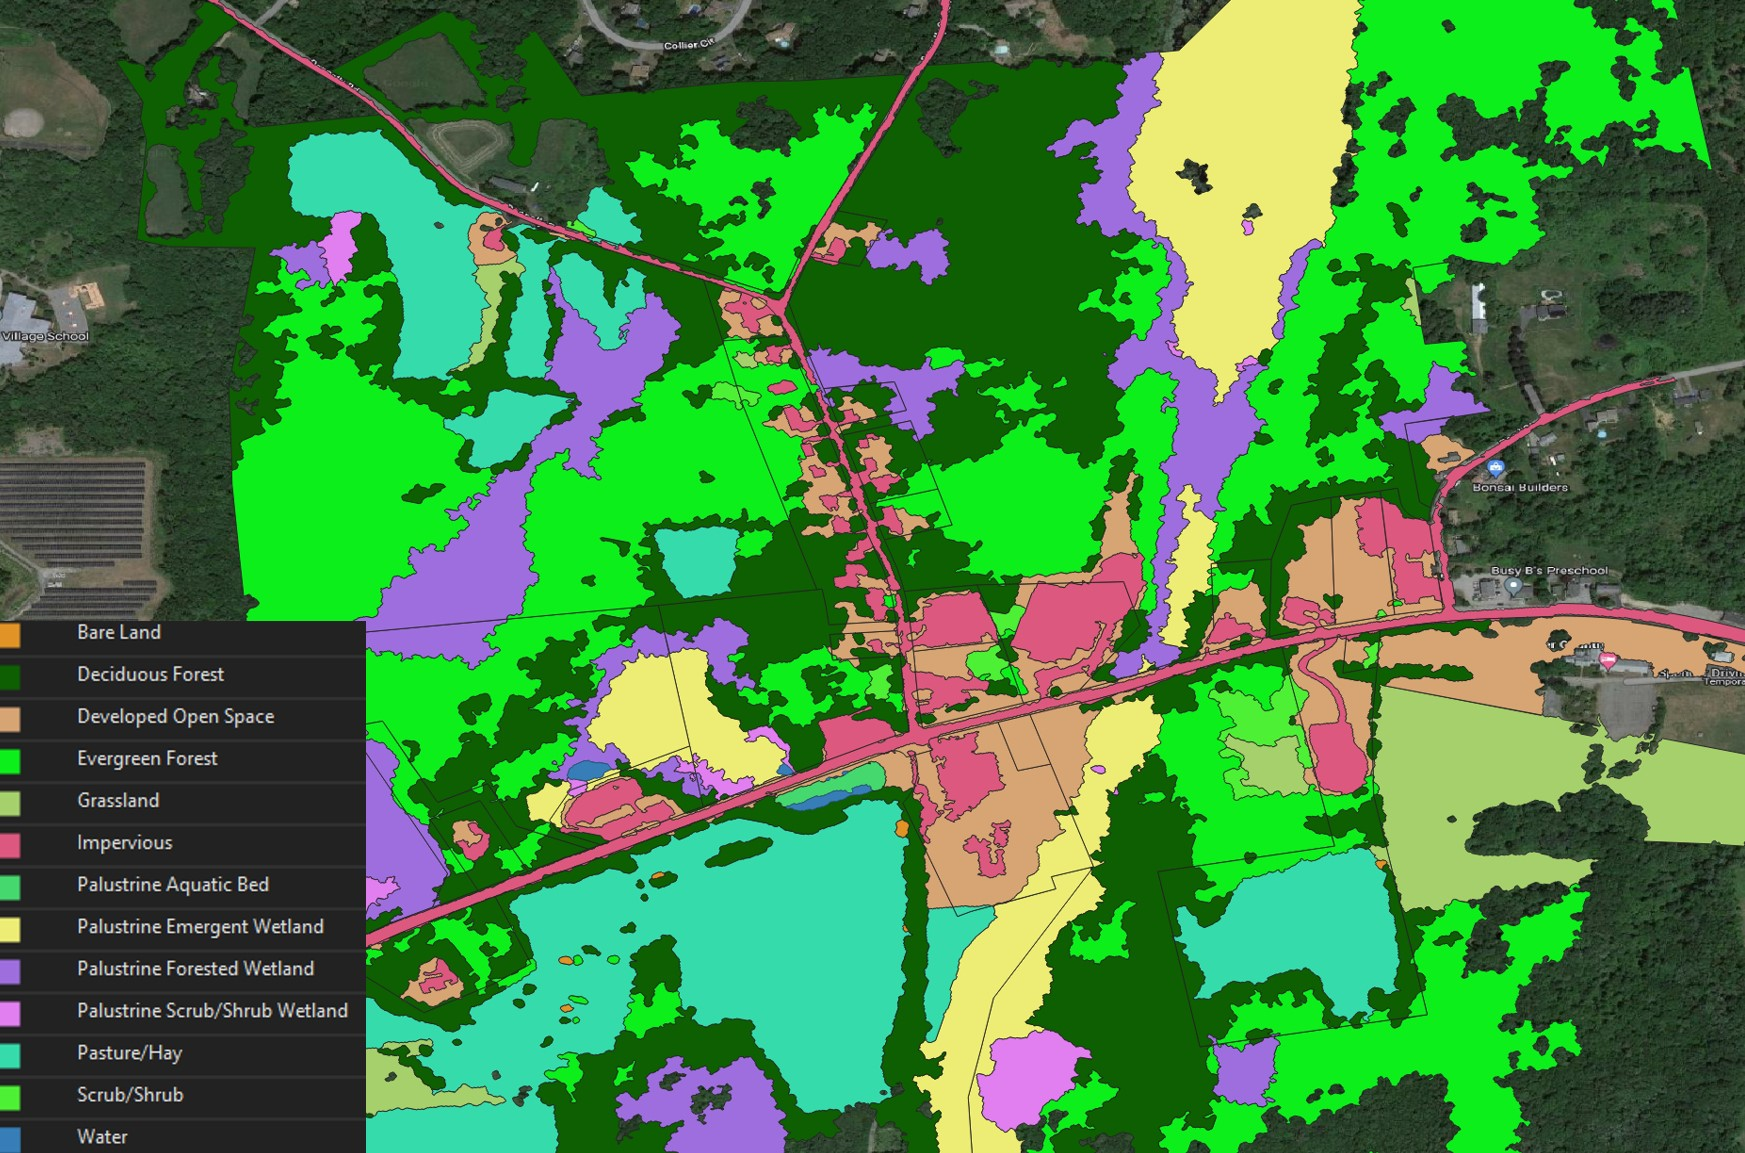
\includegraphics[width=4.5in]{landcover.jpg}
      \end{center}
\end{figure}

\begin{figure}[H]
      \caption{Building footprints}
      \begin{center}
            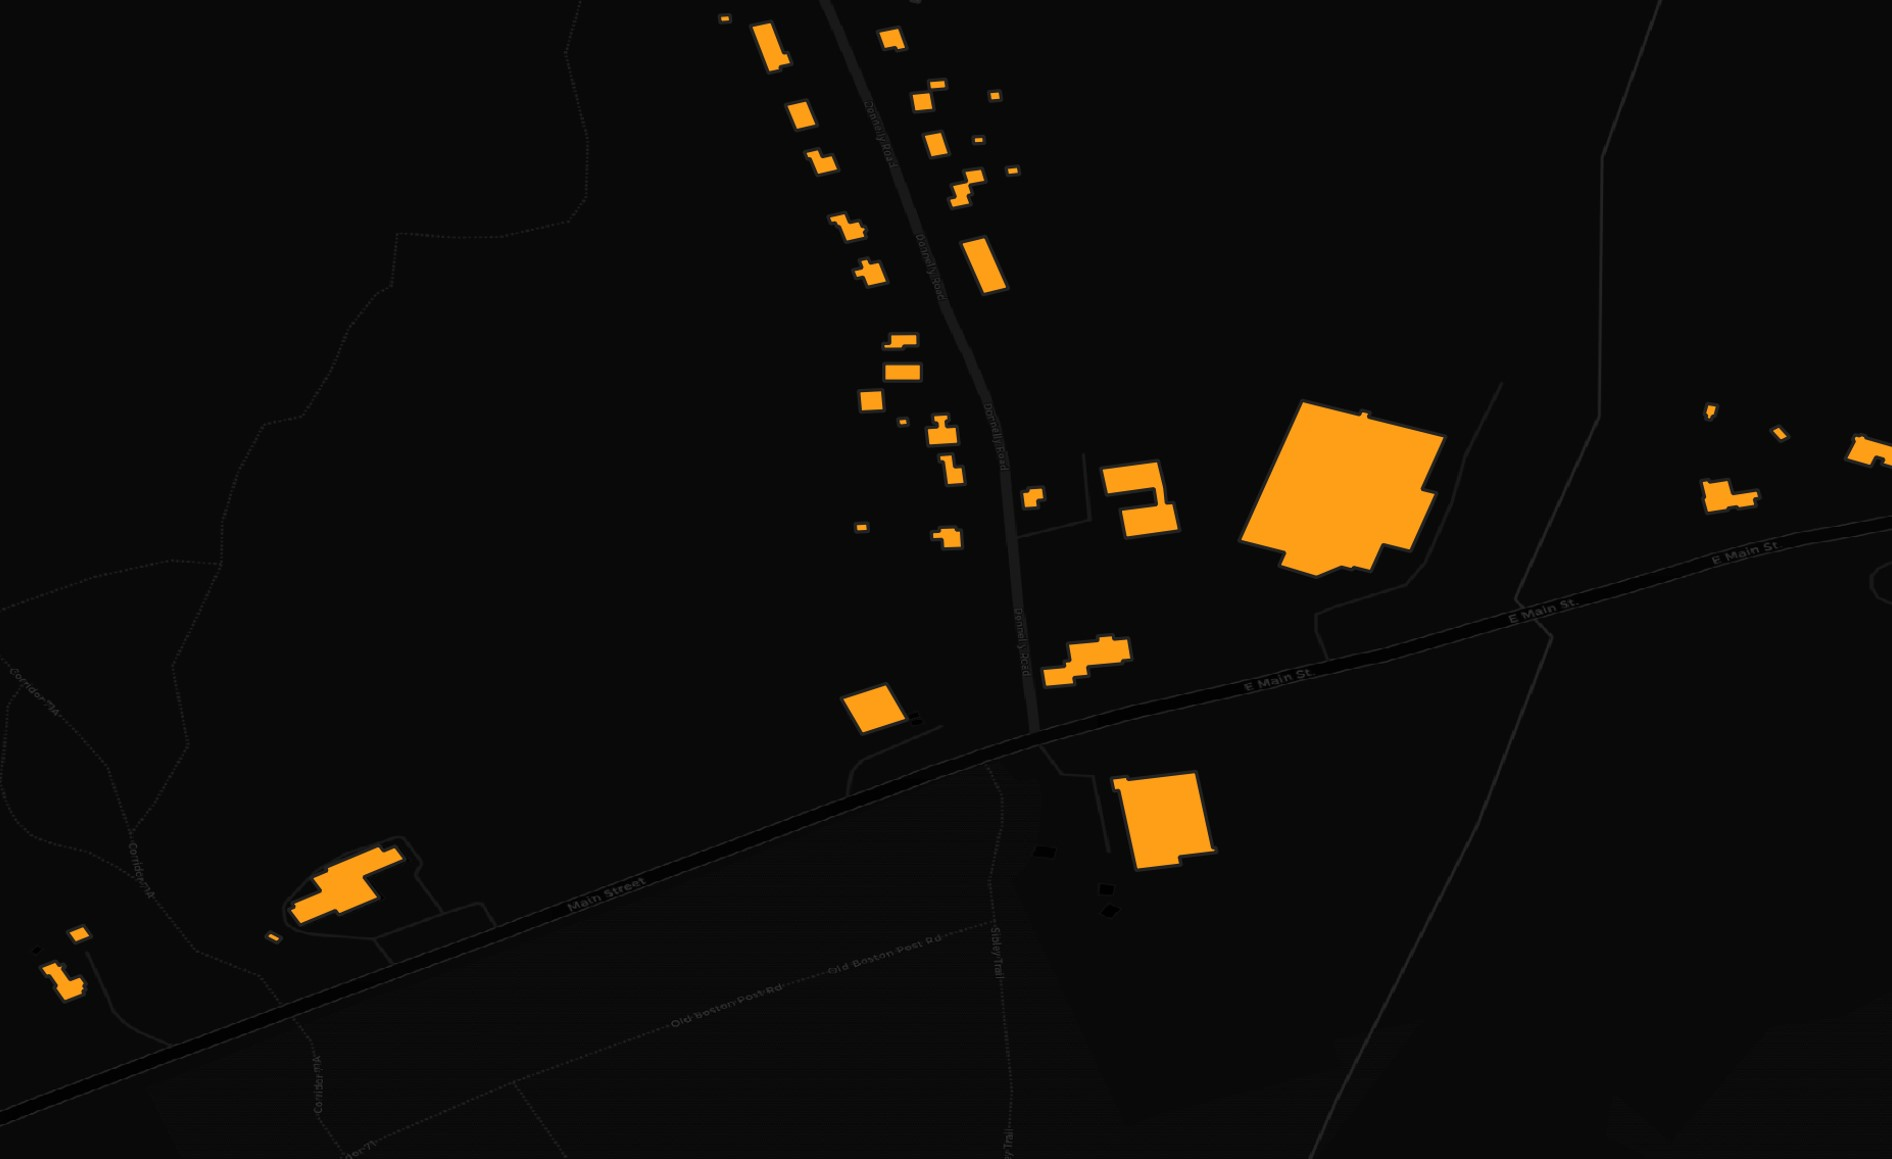
\includegraphics[width=4.5in]{buildings.jpg}
      \end{center}
\end{figure}

\begin{figure}[H]
      \caption{Tessellated bare-earth LiDAR-derived elevation}
      \begin{center}
            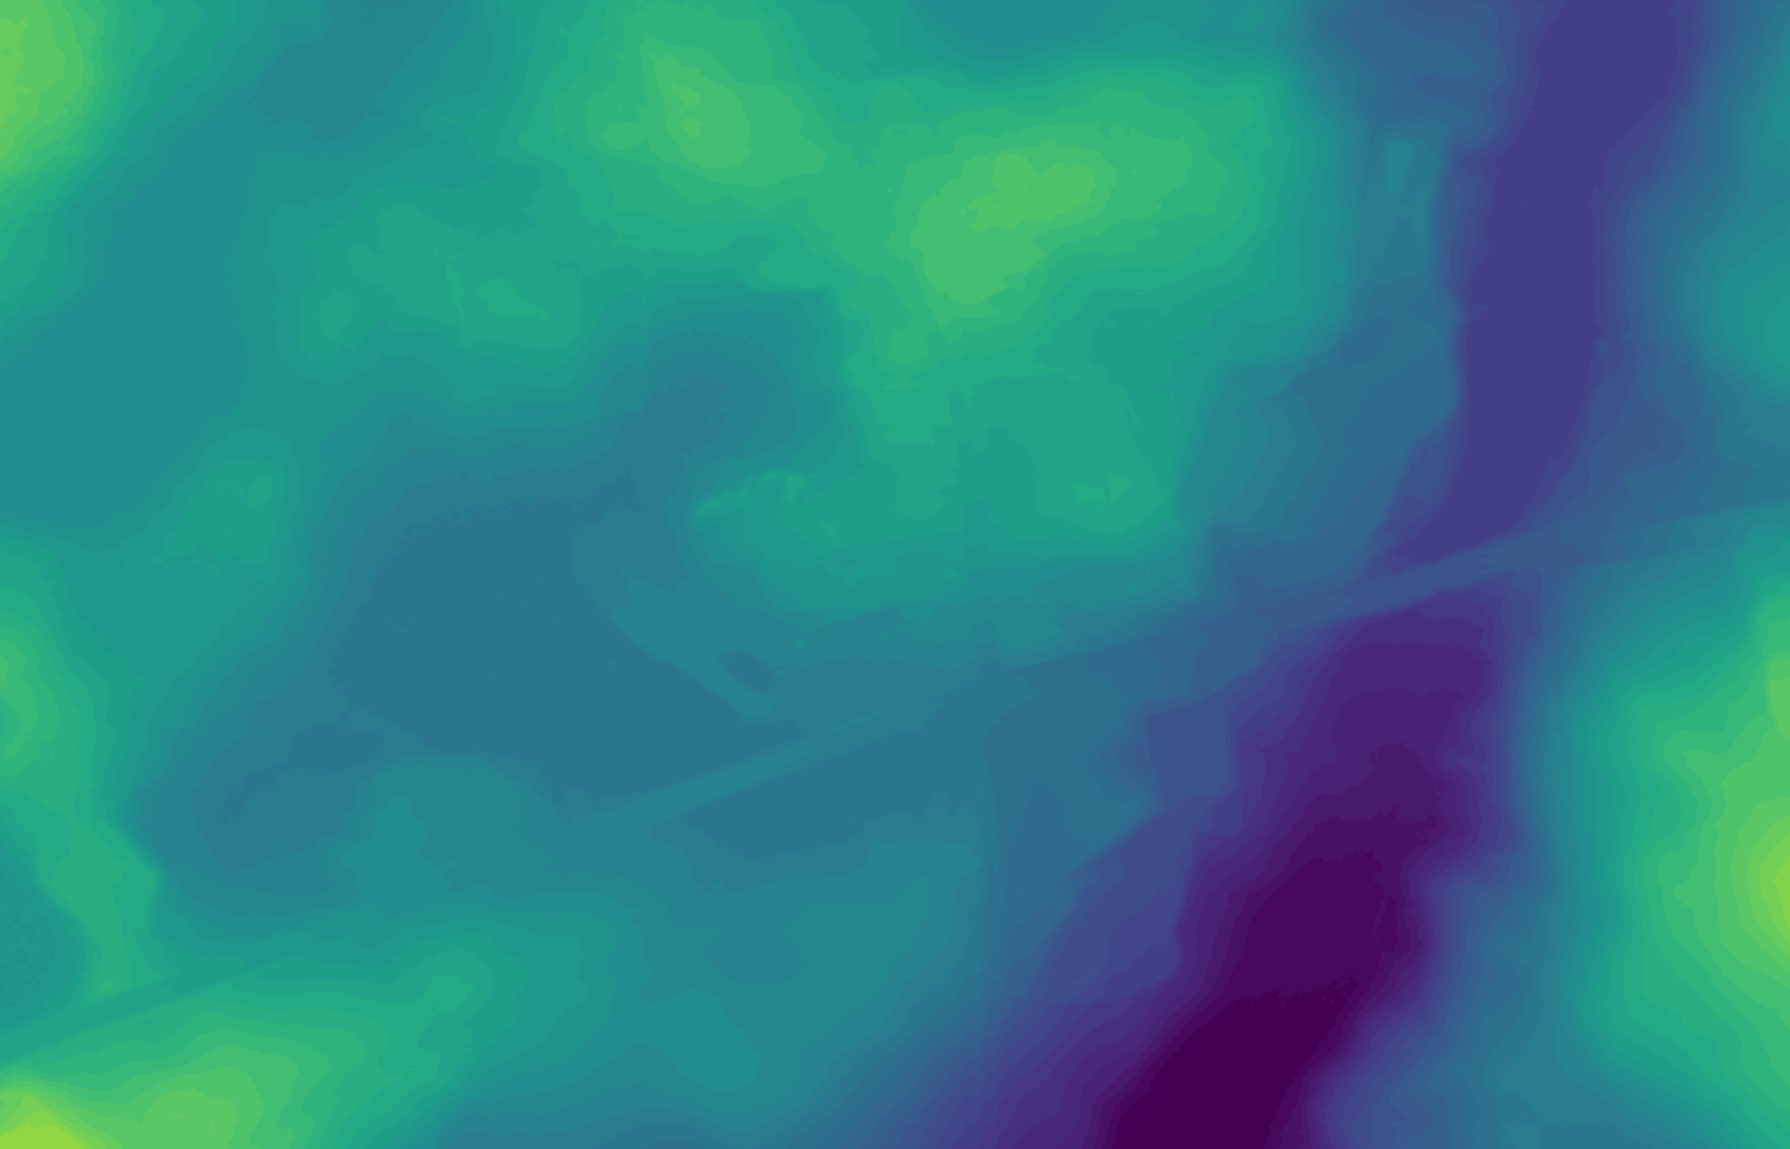
\includegraphics[width=4.5in]{bare_earth.jpg}
      \end{center}
\end{figure}

\begin{figure}[H]
      \caption{Dynamic gridded placement with Perlin noise and jittering for tree placement in forested landcover regions}
      \begin{center}
            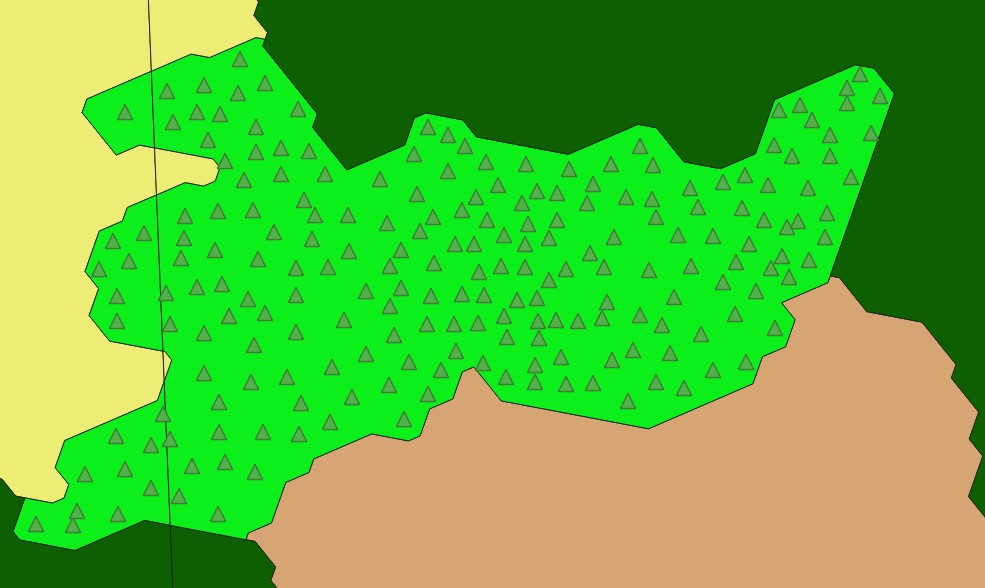
\includegraphics[width=4.5in]{tree_placement.jpg}
      \end{center}
\end{figure}

\begin{figure}[H]
      \caption{Tessellated bare-earth elevation 3D view (not yet shown as a hemisphere)}
      \begin{center}
            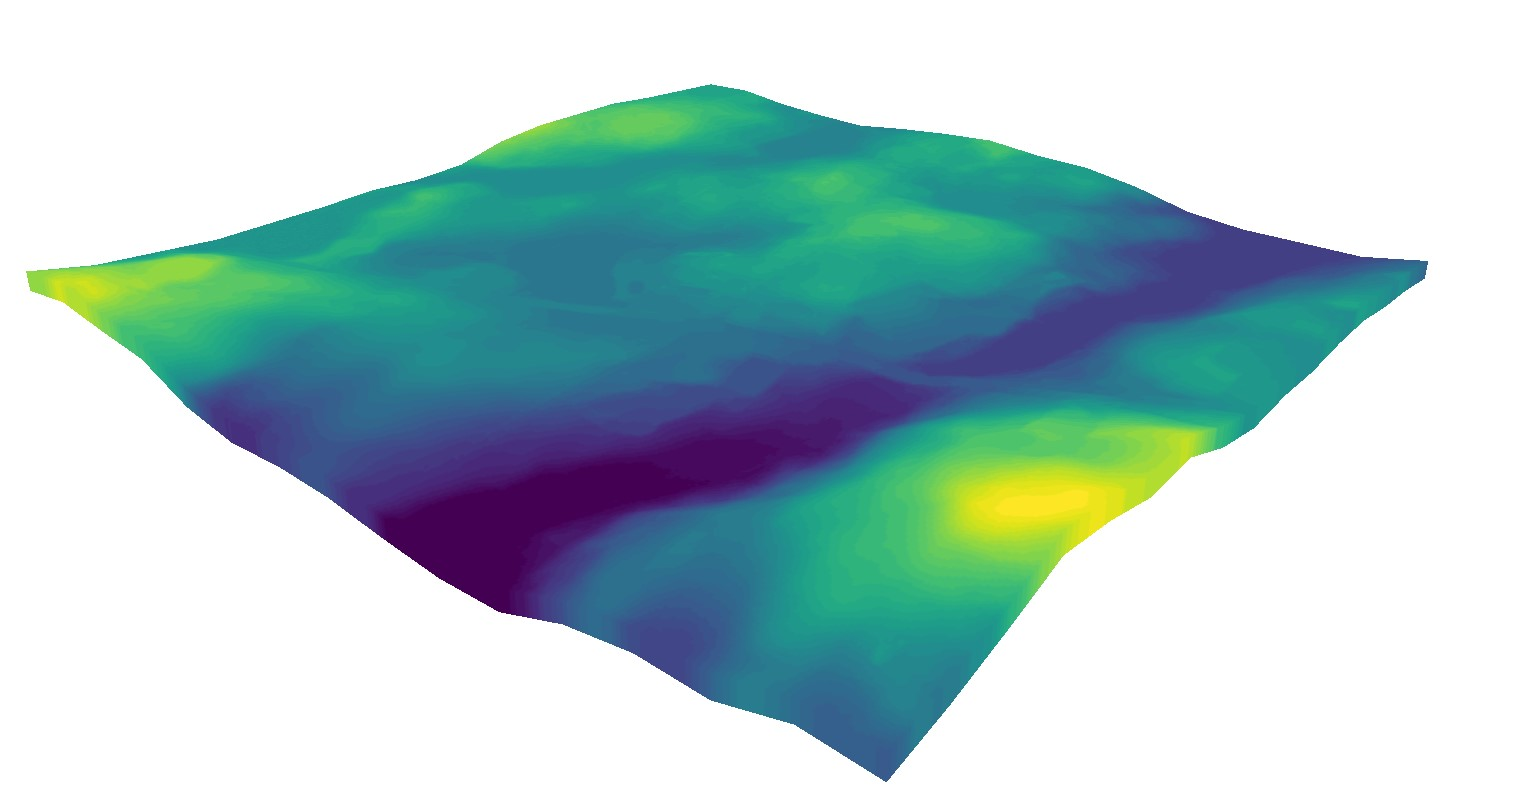
\includegraphics[width=4.5in]{terrain.jpg}
      \end{center}
\end{figure}

\section{References}

\begin{itemize}
      \item Book: The ray tracer challenge: a test-driven guide to your first 3D renderer Buck, Jamis (Access through Harvard library)

      \item MassGIS Bureau of Geographical Information

            \url{https://www.mass.gov/orgs/massgis-bureau-of-geographic-information}
      \item Ray tracing from scratch

            \url{https://raytracing.github.io/books/RayTracingInOneWeekend.html}
      \item Extracting 3D Bare-Earth Surface from Airborne LiDAR Data

            \url{https://ieeexplore.ieee.org/document/4562112} (Access through Harvard)
      \item Perlin noise generator for Python

            \url{https://pypi.org/project/perlin-noise/}
      \item Ray tracing and global illumination

            \url{https://digitalcommons.unf.edu/cgi/viewcontent.cgi?article=1100&context=ojii_volumes}

\end{itemize}


\end{document}